% OFFICIAL_REPRO_DEVELOPMENT_REPORT — built by latexmk; numbers from
% numbers.tex (auto-generated); figures from reports/figures (regenerable
% from registered JSON without model weights).
\documentclass[10pt]{article}
\usepackage[margin=2.4cm]{geometry}
\usepackage{graphicx}
\usepackage{booktabs}
\usepackage{xcolor}
\usepackage{amsmath}
\usepackage[hidelinks]{hyperref}
\usepackage{caption}
\captionsetup{font=small,labelfont=bf}
\graphicspath{{../figures/}}
% AUTO-GENERATED by jspace_official_repro.report_data — do not edit
\newcommand{\olassociationgated}{6}
\newcommand{\olassociationjlenspfive}{0.125}
\newcommand{\olassociationjlenspone}{0.083}
\newcommand{\olassociationjlensptwenty}{0.240}
\newcommand{\olassociationlogitpfive}{0.135}
\newcommand{\olassociationlogitpone}{0.073}
\newcommand{\olassociationlogitptwenty}{0.229}
\newcommand{\olassociationn}{102}
\newcommand{\olcampassociationgated}{6}
\newcommand{\olcampassociationjlenspfive}{0.125}
\newcommand{\olcampassociationjlenspone}{0.073}
\newcommand{\olcampassociationjlensptwenty}{0.229}
\newcommand{\olcampassociationlogitpfive}{0.135}
\newcommand{\olcampassociationlogitpone}{0.073}
\newcommand{\olcampassociationlogitptwenty}{0.219}
\newcommand{\olcampassociationn}{102}
\newcommand{\olcampmultihopgated}{0}
\newcommand{\olcampmultihopjlenspfive}{0.430}
\newcommand{\olcampmultihopjlenspone}{0.237}
\newcommand{\olcampmultihopjlensptwenty}{0.552}
\newcommand{\olcampmultihoplogitpfive}{0.461}
\newcommand{\olcampmultihoplogitpone}{0.220}
\newcommand{\olcampmultihoplogitptwenty}{0.606}
\newcommand{\olcampmultihopn}{93}
\newcommand{\olcampmultilingualgated}{14}
\newcommand{\olcampmultilingualjlenspfive}{0.348}
\newcommand{\olcampmultilingualjlenspone}{0.240}
\newcommand{\olcampmultilingualjlensptwenty}{0.512}
\newcommand{\olcampmultilinguallogitpfive}{0.424}
\newcommand{\olcampmultilinguallogitpone}{0.268}
\newcommand{\olcampmultilinguallogitptwenty}{0.554}
\newcommand{\olcampmultilingualn}{107}
\newcommand{\olcamporderopsgated}{0}
\newcommand{\olcamporderopsjlenspfive}{0.400}
\newcommand{\olcamporderopsjlenspone}{0.264}
\newcommand{\olcamporderopsjlensptwenty}{0.609}
\newcommand{\olcamporderopslogitpfive}{0.582}
\newcommand{\olcamporderopslogitpone}{0.400}
\newcommand{\olcamporderopslogitptwenty}{0.736}
\newcommand{\olcamporderopsn}{55}
\newcommand{\olcamppoetrygated}{0}
\newcommand{\olcamppoetryjlenspfive}{0.041}
\newcommand{\olcamppoetryjlenspone}{0.020}
\newcommand{\olcamppoetryjlensptwenty}{0.092}
\newcommand{\olcamppoetrylogitpfive}{0.041}
\newcommand{\olcamppoetrylogitpone}{0.010}
\newcommand{\olcamppoetrylogitptwenty}{0.092}
\newcommand{\olcamppoetryn}{98}
\newcommand{\olcamptypogated}{0}
\newcommand{\olcamptypojlenspfive}{0.427}
\newcommand{\olcamptypojlenspone}{0.229}
\newcommand{\olcamptypojlensptwenty}{0.667}
\newcommand{\olcamptypologitpfive}{0.542}
\newcommand{\olcamptypologitpone}{0.312}
\newcommand{\olcamptypologitptwenty}{0.688}
\newcommand{\olcamptypon}{96}
\newcommand{\olcnineassociationgated}{6}
\newcommand{\olcnineassociationjlenspfive}{0.125}
\newcommand{\olcnineassociationjlenspone}{0.062}
\newcommand{\olcnineassociationjlensptwenty}{0.219}
\newcommand{\olcnineassociationlogitpfive}{0.115}
\newcommand{\olcnineassociationlogitpone}{0.073}
\newcommand{\olcnineassociationlogitptwenty}{0.188}
\newcommand{\olcnineassociationn}{102}
\newcommand{\olcninemultihopgated}{0}
\newcommand{\olcninemultihopjlenspfive}{0.409}
\newcommand{\olcninemultihopjlenspone}{0.215}
\newcommand{\olcninemultihopjlensptwenty}{0.552}
\newcommand{\olcninemultihoplogitpfive}{0.407}
\newcommand{\olcninemultihoplogitpone}{0.220}
\newcommand{\olcninemultihoplogitptwenty}{0.579}
\newcommand{\olcninemultihopn}{93}
\newcommand{\olcninemultilingualgated}{14}
\newcommand{\olcninemultilingualjlenspfive}{0.325}
\newcommand{\olcninemultilingualjlenspone}{0.209}
\newcommand{\olcninemultilingualjlensptwenty}{0.467}
\newcommand{\olcninemultilinguallogitpfive}{0.386}
\newcommand{\olcninemultilinguallogitpone}{0.214}
\newcommand{\olcninemultilinguallogitptwenty}{0.523}
\newcommand{\olcninemultilingualn}{107}
\newcommand{\olcnineorderopsgated}{0}
\newcommand{\olcnineorderopsjlenspfive}{0.345}
\newcommand{\olcnineorderopsjlenspone}{0.218}
\newcommand{\olcnineorderopsjlensptwenty}{0.545}
\newcommand{\olcnineorderopslogitpfive}{0.473}
\newcommand{\olcnineorderopslogitpone}{0.291}
\newcommand{\olcnineorderopslogitptwenty}{0.636}
\newcommand{\olcnineorderopsn}{55}
\newcommand{\olcninepoetrygated}{0}
\newcommand{\olcninepoetryjlenspfive}{0.041}
\newcommand{\olcninepoetryjlenspone}{0.020}
\newcommand{\olcninepoetryjlensptwenty}{0.071}
\newcommand{\olcninepoetrylogitpfive}{0.041}
\newcommand{\olcninepoetrylogitpone}{0.010}
\newcommand{\olcninepoetrylogitptwenty}{0.082}
\newcommand{\olcninepoetryn}{98}
\newcommand{\olcninetypogated}{0}
\newcommand{\olcninetypojlenspfive}{0.375}
\newcommand{\olcninetypojlenspone}{0.188}
\newcommand{\olcninetypojlensptwenty}{0.583}
\newcommand{\olcninetypologitpfive}{0.438}
\newcommand{\olcninetypologitpone}{0.240}
\newcommand{\olcninetypologitptwenty}{0.656}
\newcommand{\olcninetypon}{96}
\newcommand{\olfganimacapaone}{0.0\%}
\newcommand{\olfganimacapatwo}{0.0\%}
\newcommand{\olfganimancap}{2}
\newcommand{\olfgbaseline}{40.6\%}
\newcommand{\olfgcapaone}{5.2\%}
\newcommand{\olfgcapatwo}{0.0\%}
\newcommand{\olfgcountcapaone}{0.0\%}
\newcommand{\olfgcountcapatwo}{0.0\%}
\newcommand{\olfgcountncap}{30}
\newcommand{\olfgdiagaone}{3.1\%}
\newcommand{\olfgmonthcapaone}{20.8\%}
\newcommand{\olfgmonthcapatwo}{0.0\%}
\newcommand{\olfgmonthncap}{24}
\newcommand{\olfgncapable}{68}
\newcommand{\olfgnexec}{180}
\newcommand{\olfgnumbecapaone}{0.0\%}
\newcommand{\olfgnumbecapatwo}{0.0\%}
\newcommand{\olfgnumbencap}{12}
\newcommand{\olfitdimbatch}{16}
\newcommand{\olfitmerged}{250}
\newcommand{\olfitsperprompt}{161.4}
\newcommand{\olgfold}{0.989}
\newcommand{\olhalfaassociationgated}{6}
\newcommand{\olhalfaassociationjlenspfive}{0.135}
\newcommand{\olhalfaassociationjlenspone}{0.083}
\newcommand{\olhalfaassociationjlensptwenty}{0.250}
\newcommand{\olhalfaassociationlogitpfive}{0.135}
\newcommand{\olhalfaassociationlogitpone}{0.073}
\newcommand{\olhalfaassociationlogitptwenty}{0.229}
\newcommand{\olhalfaassociationn}{102}
\newcommand{\olhalfamultihopgated}{0}
\newcommand{\olhalfamultihopjlenspfive}{0.444}
\newcommand{\olhalfamultihopjlenspone}{0.247}
\newcommand{\olhalfamultihopjlensptwenty}{0.552}
\newcommand{\olhalfamultihoplogitpfive}{0.461}
\newcommand{\olhalfamultihoplogitpone}{0.231}
\newcommand{\olhalfamultihoplogitptwenty}{0.590}
\newcommand{\olhalfamultihopn}{93}
\newcommand{\olhalfamultilingualgated}{14}
\newcommand{\olhalfamultilingualjlenspfive}{0.348}
\newcommand{\olhalfamultilingualjlenspone}{0.250}
\newcommand{\olhalfamultilingualjlensptwenty}{0.505}
\newcommand{\olhalfamultilinguallogitpfive}{0.417}
\newcommand{\olhalfamultilinguallogitpone}{0.267}
\newcommand{\olhalfamultilinguallogitptwenty}{0.560}
\newcommand{\olhalfamultilingualn}{107}
\newcommand{\olhalfaorderopsgated}{0}
\newcommand{\olhalfaorderopsjlenspfive}{0.400}
\newcommand{\olhalfaorderopsjlenspone}{0.227}
\newcommand{\olhalfaorderopsjlensptwenty}{0.582}
\newcommand{\olhalfaorderopslogitpfive}{0.582}
\newcommand{\olhalfaorderopslogitpone}{0.400}
\newcommand{\olhalfaorderopslogitptwenty}{0.736}
\newcommand{\olhalfaorderopsn}{55}
\newcommand{\olhalfapoetrygated}{0}
\newcommand{\olhalfapoetryjlenspfive}{0.041}
\newcommand{\olhalfapoetryjlenspone}{0.020}
\newcommand{\olhalfapoetryjlensptwenty}{0.092}
\newcommand{\olhalfapoetrylogitpfive}{0.041}
\newcommand{\olhalfapoetrylogitpone}{0.010}
\newcommand{\olhalfapoetrylogitptwenty}{0.082}
\newcommand{\olhalfapoetryn}{98}
\newcommand{\olhalfatypogated}{0}
\newcommand{\olhalfatypojlenspfive}{0.427}
\newcommand{\olhalfatypojlenspone}{0.208}
\newcommand{\olhalfatypojlensptwenty}{0.635}
\newcommand{\olhalfatypologitpfive}{0.542}
\newcommand{\olhalfatypologitpone}{0.312}
\newcommand{\olhalfatypologitptwenty}{0.688}
\newcommand{\olhalfatypon}{96}
\newcommand{\olhalfbassociationgated}{6}
\newcommand{\olhalfbassociationjlenspfive}{0.125}
\newcommand{\olhalfbassociationjlenspone}{0.083}
\newcommand{\olhalfbassociationjlensptwenty}{0.250}
\newcommand{\olhalfbassociationlogitpfive}{0.135}
\newcommand{\olhalfbassociationlogitpone}{0.073}
\newcommand{\olhalfbassociationlogitptwenty}{0.229}
\newcommand{\olhalfbassociationn}{102}
\newcommand{\olhalfbmultihopgated}{0}
\newcommand{\olhalfbmultihopjlenspfive}{0.444}
\newcommand{\olhalfbmultihopjlenspone}{0.258}
\newcommand{\olhalfbmultihopjlensptwenty}{0.563}
\newcommand{\olhalfbmultihoplogitpfive}{0.461}
\newcommand{\olhalfbmultihoplogitpone}{0.231}
\newcommand{\olhalfbmultihoplogitptwenty}{0.590}
\newcommand{\olhalfbmultihopn}{93}
\newcommand{\olhalfbmultilingualgated}{14}
\newcommand{\olhalfbmultilingualjlenspfive}{0.357}
\newcommand{\olhalfbmultilingualjlenspone}{0.253}
\newcommand{\olhalfbmultilingualjlensptwenty}{0.519}
\newcommand{\olhalfbmultilinguallogitpfive}{0.417}
\newcommand{\olhalfbmultilinguallogitpone}{0.267}
\newcommand{\olhalfbmultilinguallogitptwenty}{0.560}
\newcommand{\olhalfbmultilingualn}{107}
\newcommand{\olhalfborderopsgated}{0}
\newcommand{\olhalfborderopsjlenspfive}{0.391}
\newcommand{\olhalfborderopsjlenspone}{0.218}
\newcommand{\olhalfborderopsjlensptwenty}{0.582}
\newcommand{\olhalfborderopslogitpfive}{0.582}
\newcommand{\olhalfborderopslogitpone}{0.400}
\newcommand{\olhalfborderopslogitptwenty}{0.736}
\newcommand{\olhalfborderopsn}{55}
\newcommand{\olhalfbpoetrygated}{0}
\newcommand{\olhalfbpoetryjlenspfive}{0.041}
\newcommand{\olhalfbpoetryjlenspone}{0.020}
\newcommand{\olhalfbpoetryjlensptwenty}{0.092}
\newcommand{\olhalfbpoetrylogitpfive}{0.041}
\newcommand{\olhalfbpoetrylogitpone}{0.010}
\newcommand{\olhalfbpoetrylogitptwenty}{0.082}
\newcommand{\olhalfbpoetryn}{98}
\newcommand{\olhalfbtypogated}{0}
\newcommand{\olhalfbtypojlenspfive}{0.427}
\newcommand{\olhalfbtypojlenspone}{0.198}
\newcommand{\olhalfbtypojlensptwenty}{0.604}
\newcommand{\olhalfbtypologitpfive}{0.542}
\newcommand{\olhalfbtypologitpone}{0.312}
\newcommand{\olhalfbtypologitptwenty}{0.688}
\newcommand{\olhalfbtypon}{96}
\newcommand{\olmnineassociationgated}{6}
\newcommand{\olmnineassociationjlenspfive}{0.115}
\newcommand{\olmnineassociationjlenspone}{0.062}
\newcommand{\olmnineassociationjlensptwenty}{0.219}
\newcommand{\olmnineassociationlogitpfive}{0.115}
\newcommand{\olmnineassociationlogitpone}{0.073}
\newcommand{\olmnineassociationlogitptwenty}{0.188}
\newcommand{\olmnineassociationn}{102}
\newcommand{\olmninemultihopgated}{0}
\newcommand{\olmninemultihopjlenspfive}{0.409}
\newcommand{\olmninemultihopjlenspone}{0.215}
\newcommand{\olmninemultihopjlensptwenty}{0.547}
\newcommand{\olmninemultihoplogitpfive}{0.407}
\newcommand{\olmninemultihoplogitpone}{0.220}
\newcommand{\olmninemultihoplogitptwenty}{0.579}
\newcommand{\olmninemultihopn}{93}
\newcommand{\olmninemultilingualgated}{14}
\newcommand{\olmninemultilingualjlenspfive}{0.327}
\newcommand{\olmninemultilingualjlenspone}{0.224}
\newcommand{\olmninemultilingualjlensptwenty}{0.463}
\newcommand{\olmninemultilinguallogitpfive}{0.386}
\newcommand{\olmninemultilinguallogitpone}{0.214}
\newcommand{\olmninemultilinguallogitptwenty}{0.523}
\newcommand{\olmninemultilingualn}{107}
\newcommand{\olmnineorderopsgated}{0}
\newcommand{\olmnineorderopsjlenspfive}{0.327}
\newcommand{\olmnineorderopsjlenspone}{0.200}
\newcommand{\olmnineorderopsjlensptwenty}{0.555}
\newcommand{\olmnineorderopslogitpfive}{0.473}
\newcommand{\olmnineorderopslogitpone}{0.291}
\newcommand{\olmnineorderopslogitptwenty}{0.636}
\newcommand{\olmnineorderopsn}{55}
\newcommand{\olmninepoetrygated}{0}
\newcommand{\olmninepoetryjlenspfive}{0.041}
\newcommand{\olmninepoetryjlenspone}{0.020}
\newcommand{\olmninepoetryjlensptwenty}{0.071}
\newcommand{\olmninepoetrylogitpfive}{0.041}
\newcommand{\olmninepoetrylogitpone}{0.010}
\newcommand{\olmninepoetrylogitptwenty}{0.082}
\newcommand{\olmninepoetryn}{98}
\newcommand{\olmninetypogated}{0}
\newcommand{\olmninetypojlenspfive}{0.365}
\newcommand{\olmninetypojlenspone}{0.146}
\newcommand{\olmninetypojlensptwenty}{0.542}
\newcommand{\olmninetypologitpfive}{0.438}
\newcommand{\olmninetypologitpone}{0.240}
\newcommand{\olmninetypologitptwenty}{0.656}
\newcommand{\olmninetypon}{96}
\newcommand{\olmultihopgated}{0}
\newcommand{\olmultihopjlenspfive}{0.444}
\newcommand{\olmultihopjlenspone}{0.247}
\newcommand{\olmultihopjlensptwenty}{0.563}
\newcommand{\olmultihoplogitpfive}{0.461}
\newcommand{\olmultihoplogitpone}{0.231}
\newcommand{\olmultihoplogitptwenty}{0.590}
\newcommand{\olmultihopn}{93}
\newcommand{\olmultilingualgated}{14}
\newcommand{\olmultilingualjlenspfive}{0.350}
\newcommand{\olmultilingualjlenspone}{0.250}
\newcommand{\olmultilingualjlensptwenty}{0.511}
\newcommand{\olmultilinguallogitpfive}{0.417}
\newcommand{\olmultilinguallogitpone}{0.267}
\newcommand{\olmultilinguallogitptwenty}{0.560}
\newcommand{\olmultilingualn}{107}
\newcommand{\olorderopsgated}{0}
\newcommand{\olorderopsjlenspfive}{0.391}
\newcommand{\olorderopsjlenspone}{0.227}
\newcommand{\olorderopsjlensptwenty}{0.582}
\newcommand{\olorderopslogitpfive}{0.582}
\newcommand{\olorderopslogitpone}{0.400}
\newcommand{\olorderopslogitptwenty}{0.736}
\newcommand{\olorderopsn}{55}
\newcommand{\olparity}{0.0e+00}
\newcommand{\olpoetrygated}{0}
\newcommand{\olpoetryjlenspfive}{0.041}
\newcommand{\olpoetryjlenspone}{0.020}
\newcommand{\olpoetryjlensptwenty}{0.092}
\newcommand{\olpoetrylogitpfive}{0.041}
\newcommand{\olpoetrylogitpone}{0.010}
\newcommand{\olpoetrylogitptwenty}{0.082}
\newcommand{\olpoetryn}{98}
\newcommand{\olpscaptopone}{9.3\%}
\newcommand{\olpsdiagtopone}{10.7\%}
\newcommand{\olpsmulti}{9.1\%}
\newcommand{\olpsncap}{43}
\newcommand{\olpsnexec}{84}
\newcommand{\olpsnonmulti}{9.4\%}
\newcommand{\olpsntokgated}{6}
\newcommand{\olshbandfrob}{7.5\%}
\newcommand{\olshmedfrob}{8.8\%}
\newcommand{\oltypogated}{0}
\newcommand{\oltypojlenspfive}{0.427}
\newcommand{\oltypojlenspone}{0.208}
\newcommand{\oltypojlensptwenty}{0.625}
\newcommand{\oltypologitpfive}{0.542}
\newcommand{\oltypologitpone}{0.312}
\newcommand{\oltypologitptwenty}{0.688}
\newcommand{\oltypon}{96}
\newcommand{\olvrcattopfive}{25.5\%}
\newcommand{\olvrcattopone}{4.8\%}
\newcommand{\olvrimproved}{88}
\newcommand{\olvrncat}{14}
\newcommand{\olvrnexec}{118}
\newcommand{\olvrtrialtopone}{5.1\%}
\newcommand{\olvrworsened}{27}
\newcommand{\qwallassociationgated}{0}
\newcommand{\qwallassociationjlenspfive}{0.059}
\newcommand{\qwallassociationjlenspone}{0.039}
\newcommand{\qwallassociationjlensptwenty}{0.118}
\newcommand{\qwallassociationlogitpfive}{0.088}
\newcommand{\qwallassociationlogitpone}{0.020}
\newcommand{\qwallassociationlogitptwenty}{0.147}
\newcommand{\qwallassociationn}{102}
\newcommand{\qwallmultihopgated}{9}
\newcommand{\qwallmultihopjlenspfive}{0.506}
\newcommand{\qwallmultihopjlenspone}{0.286}
\newcommand{\qwallmultihopjlensptwenty}{0.730}
\newcommand{\qwallmultihoplogitpfive}{0.470}
\newcommand{\qwallmultihoplogitpone}{0.244}
\newcommand{\qwallmultihoplogitptwenty}{0.631}
\newcommand{\qwallmultihopn}{93}
\newcommand{\qwallmultilingualgated}{2}
\newcommand{\qwallmultilingualjlenspfive}{0.449}
\newcommand{\qwallmultilingualjlenspone}{0.272}
\newcommand{\qwallmultilingualjlensptwenty}{0.604}
\newcommand{\qwallmultilinguallogitpfive}{0.382}
\newcommand{\qwallmultilinguallogitpone}{0.245}
\newcommand{\qwallmultilinguallogitptwenty}{0.563}
\newcommand{\qwallmultilingualn}{107}
\newcommand{\qwallorderopsgated}{1}
\newcommand{\qwallorderopsjlenspfive}{0.600}
\newcommand{\qwallorderopsjlenspone}{0.227}
\newcommand{\qwallorderopsjlensptwenty}{0.800}
\newcommand{\qwallorderopslogitpfive}{0.673}
\newcommand{\qwallorderopslogitpone}{0.227}
\newcommand{\qwallorderopslogitptwenty}{0.800}
\newcommand{\qwallorderopsn}{55}
\newcommand{\qwallpoetrygated}{0}
\newcommand{\qwallpoetryjlenspfive}{0.020}
\newcommand{\qwallpoetryjlenspone}{0.010}
\newcommand{\qwallpoetryjlensptwenty}{0.071}
\newcommand{\qwallpoetrylogitpfive}{0.041}
\newcommand{\qwallpoetrylogitpone}{0.041}
\newcommand{\qwallpoetrylogitptwenty}{0.082}
\newcommand{\qwallpoetryn}{98}
\newcommand{\qwalltypogated}{0}
\newcommand{\qwalltypojlenspfive}{0.312}
\newcommand{\qwalltypojlenspone}{0.156}
\newcommand{\qwalltypojlensptwenty}{0.521}
\newcommand{\qwalltypologitpfive}{0.635}
\newcommand{\qwalltypologitpone}{0.406}
\newcommand{\qwalltypologitptwenty}{0.802}
\newcommand{\qwalltypon}{96}
\newcommand{\qwassociationgated}{0}
\newcommand{\qwassociationjlenspfive}{0.059}
\newcommand{\qwassociationjlenspone}{0.039}
\newcommand{\qwassociationjlensptwenty}{0.108}
\newcommand{\qwassociationlogitpfive}{0.059}
\newcommand{\qwassociationlogitpone}{0.010}
\newcommand{\qwassociationlogitptwenty}{0.118}
\newcommand{\qwassociationn}{102}
\newcommand{\qwfganimacapaone}{0.0\%}
\newcommand{\qwfganimacapatwo}{0.0\%}
\newcommand{\qwfganimancap}{6}
\newcommand{\qwfgbaseline}{51.6\%}
\newcommand{\qwfgcapaone}{5.8\%}
\newcommand{\qwfgcapatwo}{0.0\%}
\newcommand{\qwfgcountcapaone}{23.3\%}
\newcommand{\qwfgcountcapatwo}{0.0\%}
\newcommand{\qwfgcountncap}{30}
\newcommand{\qwfgdiagaone}{5.6\%}
\newcommand{\qwfgmonthcapaone}{0.0\%}
\newcommand{\qwfgmonthcapatwo}{0.0\%}
\newcommand{\qwfgmonthncap}{18}
\newcommand{\qwfgncapable}{78}
\newcommand{\qwfgnexec}{180}
\newcommand{\qwfgnumbecapaone}{0.0\%}
\newcommand{\qwfgnumbecapatwo}{0.0\%}
\newcommand{\qwfgnumbencap}{24}
\newcommand{\qwgfold}{0.382}
\newcommand{\qwmultihopgated}{9}
\newcommand{\qwmultihopjlenspfive}{0.399}
\newcommand{\qwmultihopjlenspone}{0.244}
\newcommand{\qwmultihopjlensptwenty}{0.641}
\newcommand{\qwmultihoplogitpfive}{0.327}
\newcommand{\qwmultihoplogitpone}{0.173}
\newcommand{\qwmultihoplogitptwenty}{0.542}
\newcommand{\qwmultihopn}{93}
\newcommand{\qwmultilingualgated}{2}
\newcommand{\qwmultilingualjlenspfive}{0.384}
\newcommand{\qwmultilingualjlenspone}{0.237}
\newcommand{\qwmultilingualjlensptwenty}{0.580}
\newcommand{\qwmultilinguallogitpfive}{0.327}
\newcommand{\qwmultilinguallogitpone}{0.184}
\newcommand{\qwmultilinguallogitptwenty}{0.497}
\newcommand{\qwmultilingualn}{107}
\newcommand{\qworderopsgated}{1}
\newcommand{\qworderopsjlenspfive}{0.455}
\newcommand{\qworderopsjlenspone}{0.145}
\newcommand{\qworderopsjlensptwenty}{0.727}
\newcommand{\qworderopslogitpfive}{0.600}
\newcommand{\qworderopslogitpone}{0.209}
\newcommand{\qworderopslogitptwenty}{0.727}
\newcommand{\qworderopsn}{55}
\newcommand{\qwparity}{0.0e+00}
\newcommand{\qwpoetrygated}{0}
\newcommand{\qwpoetryjlenspfive}{0.020}
\newcommand{\qwpoetryjlenspone}{0.010}
\newcommand{\qwpoetryjlensptwenty}{0.071}
\newcommand{\qwpoetrylogitpfive}{0.031}
\newcommand{\qwpoetrylogitpone}{0.020}
\newcommand{\qwpoetrylogitptwenty}{0.061}
\newcommand{\qwpoetryn}{98}
\newcommand{\qwpscaptopone}{14.3\%}
\newcommand{\qwpsdiagtopone}{14.5\%}
\newcommand{\qwpsmulti}{10.5\%}
\newcommand{\qwpsncap}{63}
\newcommand{\qwpsnexec}{83}
\newcommand{\qwpsnonmulti}{15.9\%}
\newcommand{\qwpsntokgated}{7}
\newcommand{\qwtypogated}{0}
\newcommand{\qwtypojlenspfive}{0.271}
\newcommand{\qwtypojlenspone}{0.135}
\newcommand{\qwtypojlensptwenty}{0.500}
\newcommand{\qwtypologitpfive}{0.594}
\newcommand{\qwtypologitpone}{0.333}
\newcommand{\qwtypologitptwenty}{0.719}
\newcommand{\qwtypon}{96}
\newcommand{\qwvrcattopfive}{0.8\%}
\newcommand{\qwvrcattopone}{0.0\%}
\newcommand{\qwvrimproved}{64}
\newcommand{\qwvrncat}{14}
\newcommand{\qwvrnexec}{118}
\newcommand{\qwvrtrialtopone}{0.0\%}
\newcommand{\qwvrworsened}{53}


\definecolor{jblue}{HTML}{2A78D6}
\definecolor{jorange}{HTML}{EB6834}
\definecolor{ink2}{HTML}{52514E}

\title{\textbf{Released-Materials Reproduction, Study 1 (\texttt{or1-})}\\
\large Running the Anthropic Jacobian-lens battery on Qwen 3.6 27B and
OLMo 3.1 32B Instruct\\
\normalsize development/methods tier --- prompt-exact where released,
method-reconstructed where specified, gated where not identified}
\author{J-space campaign --- official-repro sideline\\
\small branch \texttt{interp\_jspace\_official\_repro\_1} ---
upstream \texttt{anthropics/jacobian-lens @ 581d3986}}
\date{2026-08-08 (OR1-A Qwen block)}

\begin{document}
\maketitle

\begin{abstract}
\noindent We run the released Jacobian-lens evaluations (6 sets) and
experiment prompt sets (11 sets) from the public companion release of
``Verbalizable Representations Form a Global Workspace in Language
Models'' under one audited harness on two open-weight models, and
separate prompt, lens, intervention, capability, and model effects.
This report covers the Qwen lane: the campaign-pinned checkpoint with
the published $n{=}1000$ lens --- the study's mechanical instrument
anchor (OR-Q1) and its first generalization surface (OR-Q2). Fidelity
classes and gate states are carried on every cell; gated cells are
missing, never zero; no confirmatory language is licensed anywhere in
Study 1.
\end{abstract}

\section{Provenance and instrument identity}

\begin{table}[h]\centering\small
\begin{tabular}{ll}
\toprule
Upstream release & \texttt{anthropics/jacobian-lens} @ \texttt{581d3986} (11 experiments + 6 evals, hash-pinned)\\
Qwen checkpoint & \texttt{Qwen/Qwen3.6-27B} @ \texttt{6a9e13bd} (64 layers, $d{=}5120$, 48 GDN blocks verified)\\
Published lens & \texttt{neuronpedia/jacobian-lens} @ \texttt{a4114d7}, $n{=}1000$, sha256 \texttt{1718c8c5\ldots} byte-verified\\
Readout parity & max abs.\ diff \qwparity{} (hard stop threshold $10^{-4}$; exact top-20 order agreement)\\
$\alpha{=}0$ no-op & exact (0.0 logit difference across a full-position band session)\\
g-folding audit & min cosine \qwgfold{} over 26 battery tokens $\times$ 14 band layers --- \textbf{material}; D9: paper-literal unfolded $v_t$ stays primary\\
Bands & paper grid 25 layers; workspace band $[24,58]$; campaign band sensitivity $[20\ldots44]$\\
\bottomrule
\end{tabular}
\caption{Lane admission. The boot-probe sentinel (Fig.~\ref{fig:slice})
reads the latent country mid-band and the currency near the output ---
the instrument behaves as the paper describes before any experiment
runs.}
\end{table}

\section{The paper's own example, on Qwen}

\begin{figure}[h]\centering
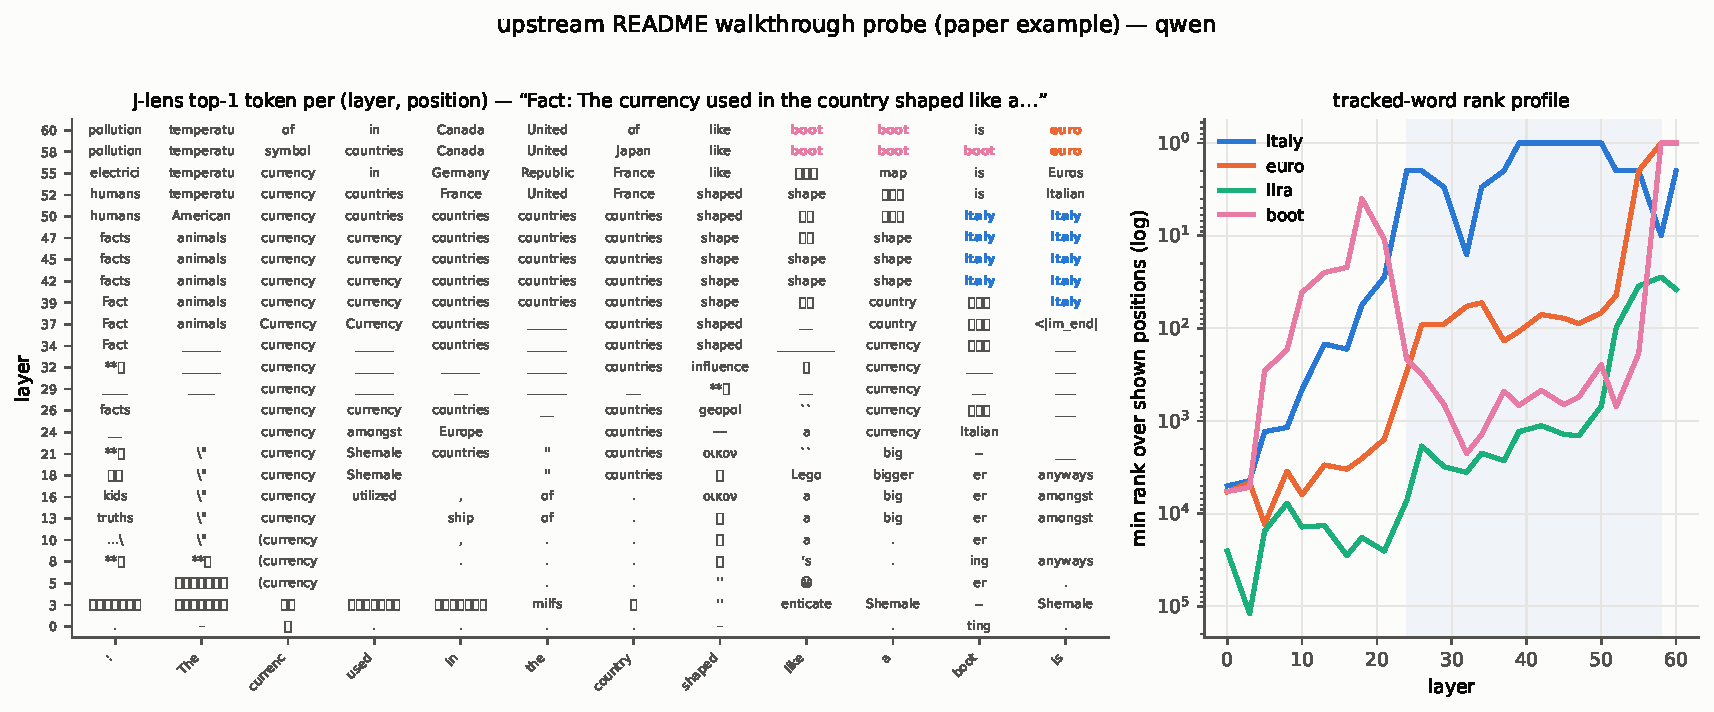
\includegraphics[width=\textwidth]{or1f06_slice_boot_qwen.pdf}
\caption{\label{fig:slice}The upstream README walkthrough probe
(``The currency used in the country shaped like a boot is'') under the
published lens on Qwen 3.6 27B. Left: J-lens top-1 token per (layer,
position); colored cells are tracked words. Right: tracked-word best
rank by layer (shaded: workspace band). \textcolor{jblue}{Italy} appears
as latent content mid-band and hands off to
\textcolor{jorange}{euro}/lira toward the output --- the paper's
slice-visualisation phenomenology, reproduced from released materials.}
\end{figure}

\begin{figure}[h]\centering
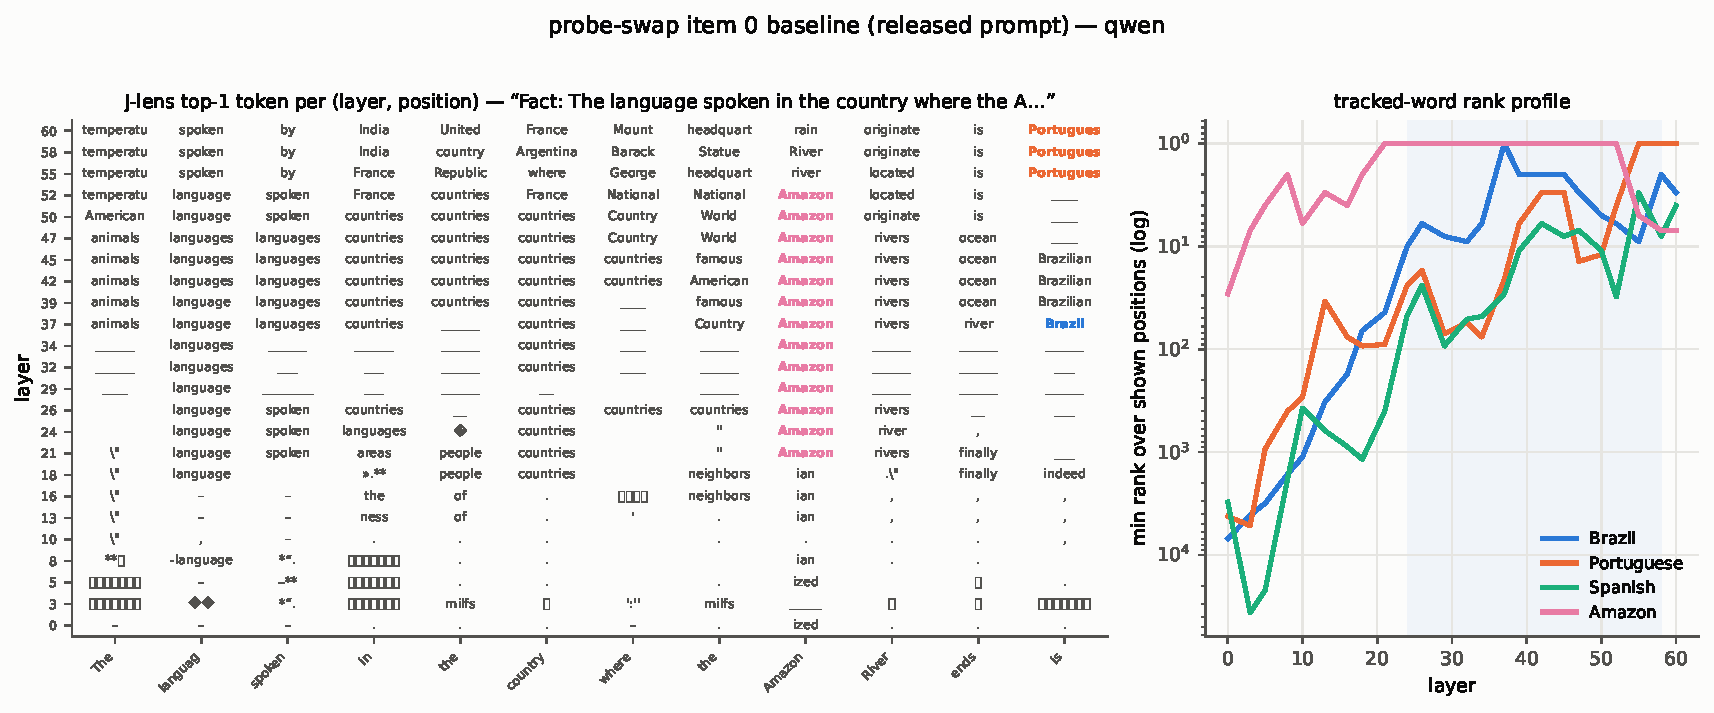
\includegraphics[width=\textwidth]{or1f07_slice_amazon_qwen.pdf}
\caption{Released probe-swap item 0 (``the language spoken in the
country where the Amazon River ends'') --- the two-hop structure is
visible: \textcolor{jblue}{Brazil} (bridge entity) carried in-band while
the output side resolves toward \textcolor{jorange}{Portuguese}.}
\end{figure}

\section{Six released lens evaluations (OR-Q1)}

\begin{figure}[h]\centering
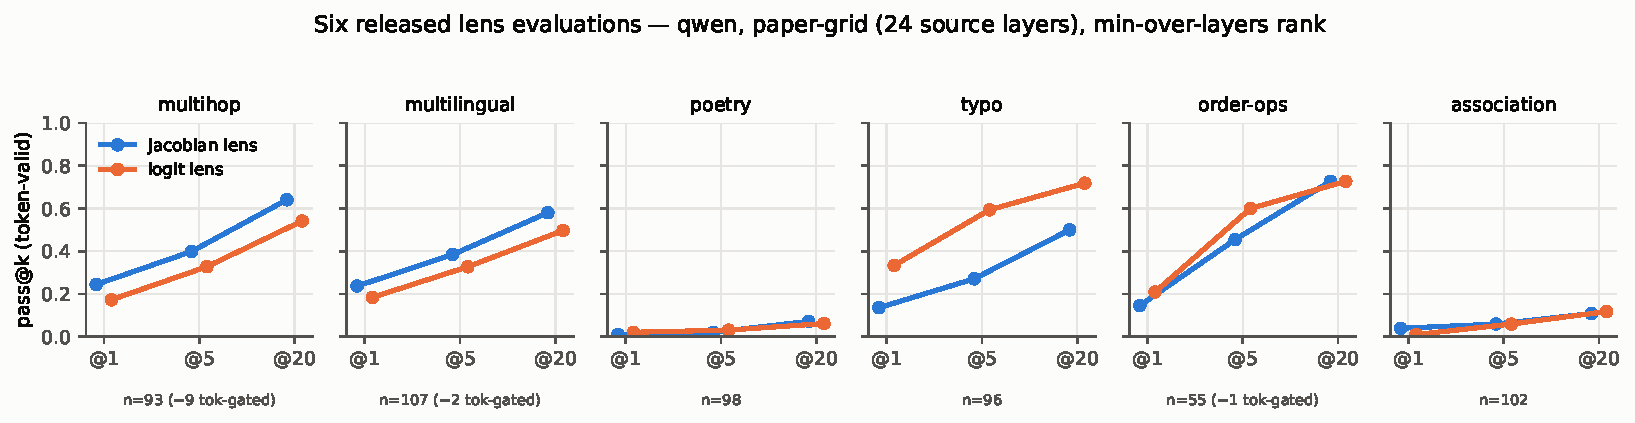
\includegraphics[width=\textwidth]{or1f01_evals_qwen.pdf}
\caption{pass@$k$ per released set, token-valid denominators,
min-over-24-paper-grid-layers at the released readout position.}
\end{figure}

\begin{figure}[h]\centering
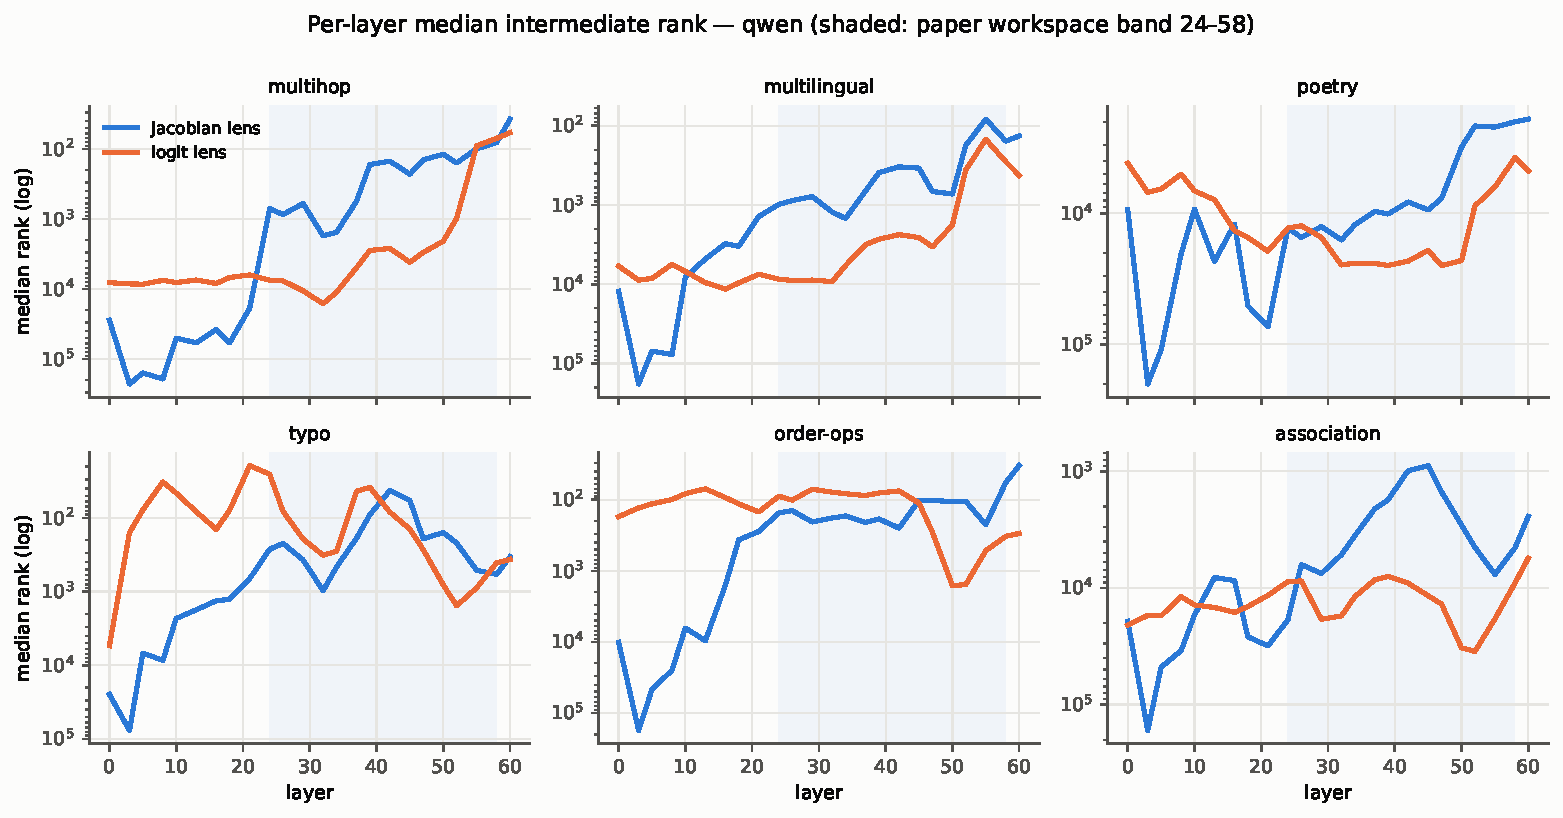
\includegraphics[width=\textwidth]{or1f02_layer_profiles_qwen.pdf}
\caption{\label{fig:profiles}Median intermediate rank by layer. On the
latent-content sets (multihop, multilingual) the J-lens reaches useful
ranks by the band onset while the logit lens remains near rank $10^4$
until $\sim$L45 --- the paper's central methods-comparison claim,
visible on an open model. On typo the logit lens is stronger (the
correction is surface-adjacent); order-ops numbers sit in the prompt, so
the logit lens copies them early.}
\end{figure}

\begin{table}[h]\centering\small
\begin{tabular}{lrrrrrr}
\toprule
& \multicolumn{3}{c}{Jacobian lens} & \multicolumn{3}{c}{logit lens}\\
Set & @1 & @5 & @20 & @1 & @5 & @20\\
\midrule
multihop ($n{=}\qwmultihopn$) & \qwmultihopjlensp1 & \qwmultihopjlensp5 & \qwmultihopjlensp20 & \qwmultihoplogitp1 & \qwmultihoplogitp5 & \qwmultihoplogitp20\\
multilingual ($n{=}\qwmultilingualn$) & \qwmultilingualjlensp1 & \qwmultilingualjlensp5 & \qwmultilingualjlensp20 & \qwmultilinguallogitp1 & \qwmultilinguallogitp5 & \qwmultilinguallogitp20\\
poetry ($n{=}\qwpoetryn$) & \qwpoetryjlensp1 & \qwpoetryjlensp5 & \qwpoetryjlensp20 & \qwpoetrylogitp1 & \qwpoetrylogitp5 & \qwpoetrylogitp20\\
typo ($n{=}\qwtypon$) & \qwtypojlensp1 & \qwtypojlensp5 & \qwtypojlensp20 & \qwtypologitp1 & \qwtypologitp5 & \qwtypologitp20\\
order-ops ($n{=}\qworderopsn$) & \qworderopsjlensp1 & \qworderopsjlensp5 & \qworderopsjlensp20 & \qworderopslogitp1 & \qworderopslogitp5 & \qworderopslogitp20\\
association ($n{=}\qwassociationn$) & \qwassociationjlensp1 & \qwassociationjlensp5 & \qwassociationjlensp20 & \qwassociationlogitp1 & \qwassociationlogitp5 & \qwassociationlogitp20\\
\bottomrule
\end{tabular}
\caption{pass@$k$, token-valid primary. All-source-layer sensitivity and
released-denominator sensitivity live in the registered JSON.}
\end{table}

\section{Qwen causal core (OR-Q2)}

\subsection{Verbal report}
Release-literal rule (first ten listed candidates, skip the answer),
swap-out = greedy token at the generation boundary (D1), $\alpha{=}1$
across the band at every prompt position. Category-equal top-1
\qwvrcattopone{} and top-5 \qwvrcattopfive{} over \qwvrncat{} categories
(\qwvrnexec{} executed trials; \qwvrimproved{} trials improved the
candidate's rank, \qwvrworsened{} worsened). Paper context (Claude):
88\% top-5. The effect on Qwen under the paper-literal operation is
\emph{directionally present in rank movement but far below the paper's
report-rate}: Fig.~\ref{fig:vr}.

\begin{figure}[h]\centering
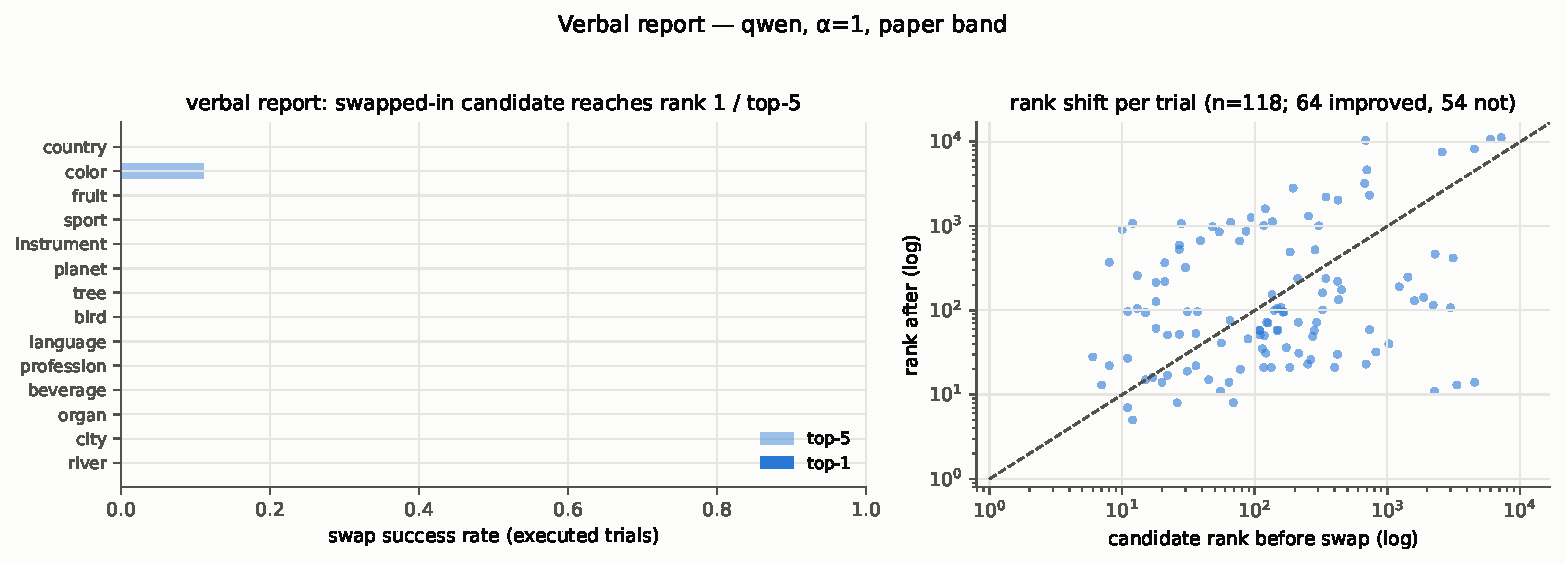
\includegraphics[width=\textwidth]{or1f03_verbal_report_qwen.pdf}
\caption{\label{fig:vr}Verbal report on Qwen: per-category success rates
(left) and per-trial rank shifts (right; below the diagonal = swap moved
the candidate toward the output).}
\end{figure}

\subsection{Flexible generalization}
All 192 ordered off-diagonal swaps; capability-conditioned primary
(source and target baselines correct; baseline accuracy
\qwfgbaseline{}); $\alpha{=}2$ full sensitivity. Category-equal
capable top-1: \qwfgcapaone{} ($\alpha{=}1$) $\to$ \qwfgcapatwo{}
($\alpha{=}2$); diagnostic all-executable: \qwfgdiagaone{}. Paper
context: $76/192 \to 101/192$ (Sonnet 4.5). Per-category grids in
Fig.~\ref{fig:fg}.

\begin{figure}[h]\centering
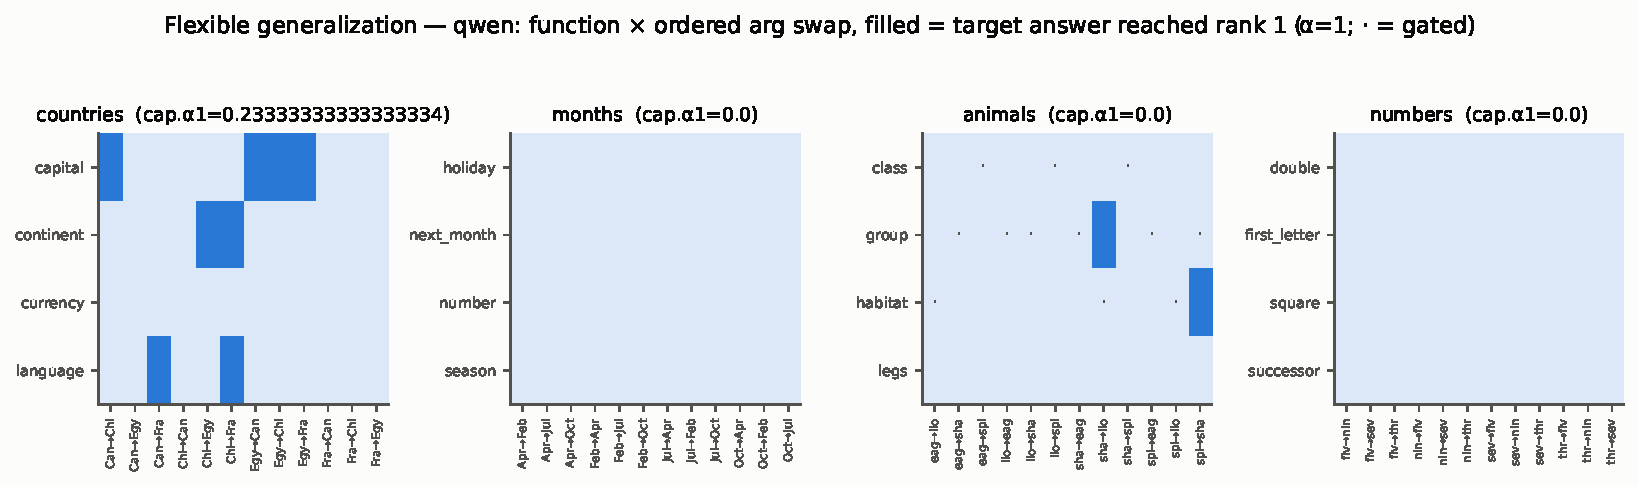
\includegraphics[width=\textwidth]{or1f04_flexgen_qwen.pdf}
\caption{\label{fig:fg}Function $\times$ ordered-argument-swap outcomes,
$\alpha{=}1$ (filled = target answer reached rank 1).}
\end{figure}

\subsection{Probe-swap, raw J-lens token arm}
Fidelity \texttt{prompt\_exact\_representation\_adapted\_raw\_jlens}
(the paper's own \S3.3 headline arm; the official linear-probe arm is
NOT-IDENTIFIED --- its training corpus is absent from the release).
Population: 90 released items, \qwpsntokgated{} tokenization-gated,
\qwpsnexec{} executed, \qwpsncap{} baseline-capable. Capable top-1
\qwpscaptopone{} (diagnostic \qwpsdiagtopone{}); multihop
\qwpsmulti{} vs non-multihop \qwpsnonmulti{}. Paper context: 60\%
(Claude, $n{=}90$).

\begin{figure}[h]\centering
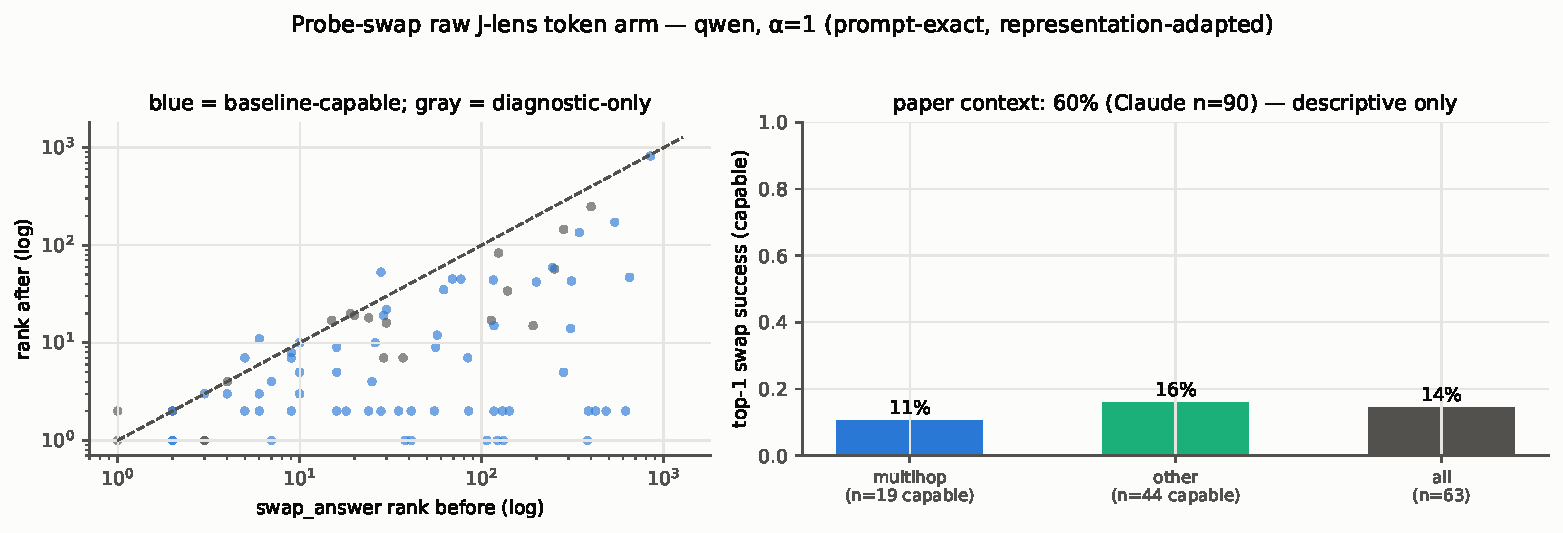
\includegraphics[width=\textwidth]{or1f05_probe_swap_qwen.pdf}
\caption{Probe-swap raw arm on Qwen: per-item rank movement of the
predicted swapped answer (left) and capable top-1 by category group
(right).}
\end{figure}

\section{Interpretation under the wording router}

Conformance and admission passed mechanically (exact parity, exact
no-ops, verified pins), so every result above is a scientific
observation about this model/instrument cell, not a harness state. The
lens-eval layer profiles reproduce the paper's methods-comparison
direction on the latent-content distributions; the paper-literal
$\alpha{=}1$ coordinate-swap core is \emph{directionally present but
substantially weaker on Qwen 3.6 27B than the paper's Claude values},
with rank movement concentrated below top-1. Maximum licensed sentence
(plan \S7.6 routing, pre-OLMo): \emph{``conformance passes; the Qwen
core is a valid generalization result''} --- the released functional
properties do not transfer at paper magnitude to this cell under
prompt-exact, method-reconstructed conditions. No workspace-existence
or -absence claim is licensed; OLMo, the extended battery, and the
instrument cross-over (which will separate intervention semantics from
prompt population) follow in OR1-B/C/D.

\section{Population accounting}

Every released row carries source-present / tokenization-valid /
geometry-valid / baseline-capable / executed states in the registered
raw records (\texttt{*\_raw.jsonl}, plan \S12 schema); the attrition
waterfall figure ships with the OLMo lane so both lanes share one
accounting frame. Nothing gated was encoded as zero anywhere in this
report.

\end{document}
